\documentclass[xetex, 20pt]{beamer}
\usepackage{amsmath, amsfonts, epsfig, xspace}
\usepackage{pstricks,pst-node}
%\usepackage[utf8]{inputenc}
\usepackage[normal,tight,center]{subfigure}
\setlength{\subfigcapskip}{-.5em}
\usepackage{beamerthemesplit}
\usepackage{listings}
\usepackage{xcolor}
\usepackage{graphicx}
\usepackage{tikz}
\usepackage{textpos}
\usetikzlibrary{patterns}
\usetheme{libjava-theme}
\newcommand{\putat}[3]{\begin{picture}(0,0)(0,0)\put(#1,#2){#3}\end{picture}} % just a shorthand
\newcommand<>{\fullsizegraphic}[3]{
  \begin{textblock*}{0cm}(#1,#2)
  \includegraphics[width=\paperwidth]{#3}
  \end{textblock*}
}

\author[Marcel Hlopko]{\footnotesize Claus Gittinger\\* Marcel Hlopko\\* Jan Kurš \\* Jan Vraný}

\title[ST/X Libjava\hspace{2em}\insertframenumber/\inserttotalframenumber]{When a Virtual Machine is not Complex Enough}

\begin{document}

\maketitle

\begin{frame}
	\frametitle{What is \libjava}
	\yeahtext{A Java implementation for Smalltalk/X}
\end{frame}

\begin{frame}
  \frametitle{Smalltalk/X}
  What is Smalltalk/X??
  \begin{itemize}
	  \item Fast smalltalk implementation \pause
	  \item VM written in C, including JIT \pause
	  \item Support for Ruby, Javascript, XQuery, Pascal
  \end{itemize}
\end{frame}

\begin{frame}
  \frametitle{\libjava}
  Why yet another language?
  \begin{itemize}
	  \item different approach \pause
	  \item possibility to reuse existing code \pause
	  \item interop research \pause
  \end{itemize}

  \putat{120}{-30}{{\yeahtext{and it's fun :)}}}
\end{frame}

\begin{frame}
	\frametitle{Hands on - JUnit}
    \pause
	\putat{-30}{-80}{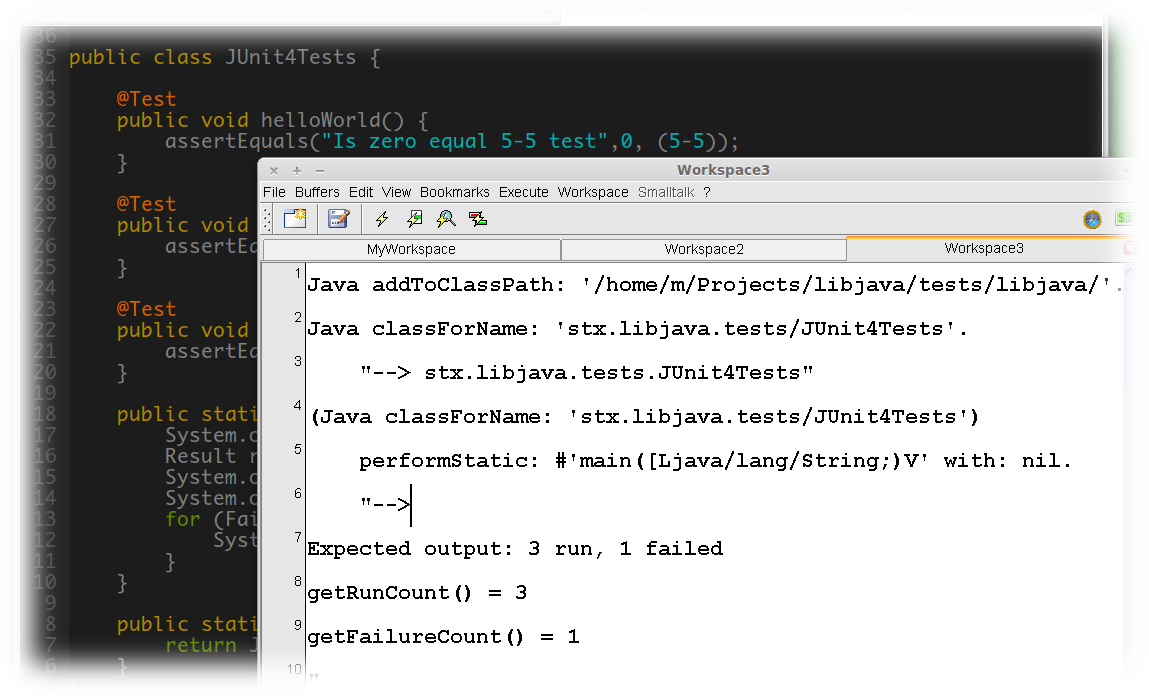
\includegraphics[width=11cm]{figures/junit-sshot.png}}
	\pause
	\putat{70}{-100}{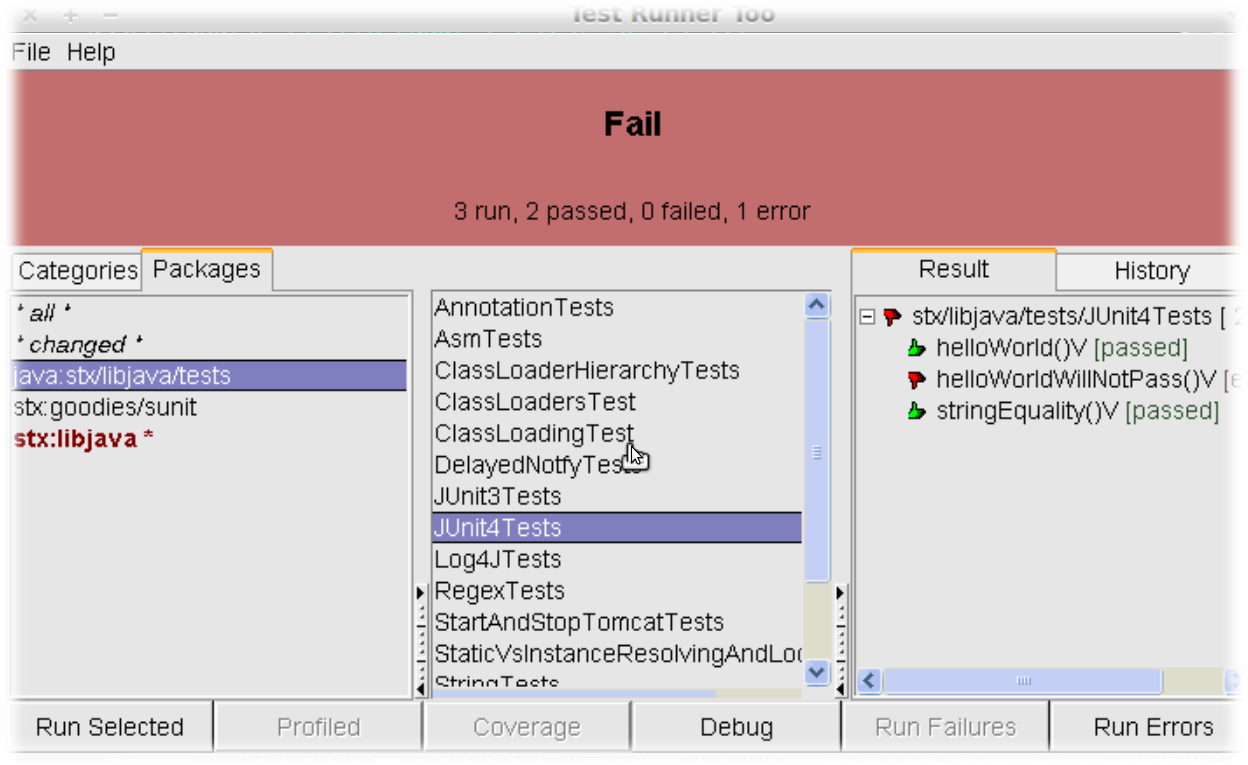
\includegraphics[width=9cm]{figures/test-runner.png}}
\end{frame}

\begin{frame}
	\frametitle{Hands on - JUnit}
	\putat{60}{-30}{{\wtftext{That's it??}}}
	\putat{190}{-90}{
\includegraphics[width=5cm]{figures/angry.png}}
	\pause
	\putat{-10}{-70}{{\yeahtext{Not quite yet}}}
\end{frame}

\begin{frame}
	\frametitle{How it works?}
	
	\begin{itemize}
		\item loads Java \texttt{.class} files \pause
		\item executes Java bytecodes (no translation)\pause
        \item no difference between Java and Smalltalk objects		
	\end{itemize}
\end{frame}

\begin{frame}
  \frametitle{High level overview}
  \begin{figure}[t]
	\centering
	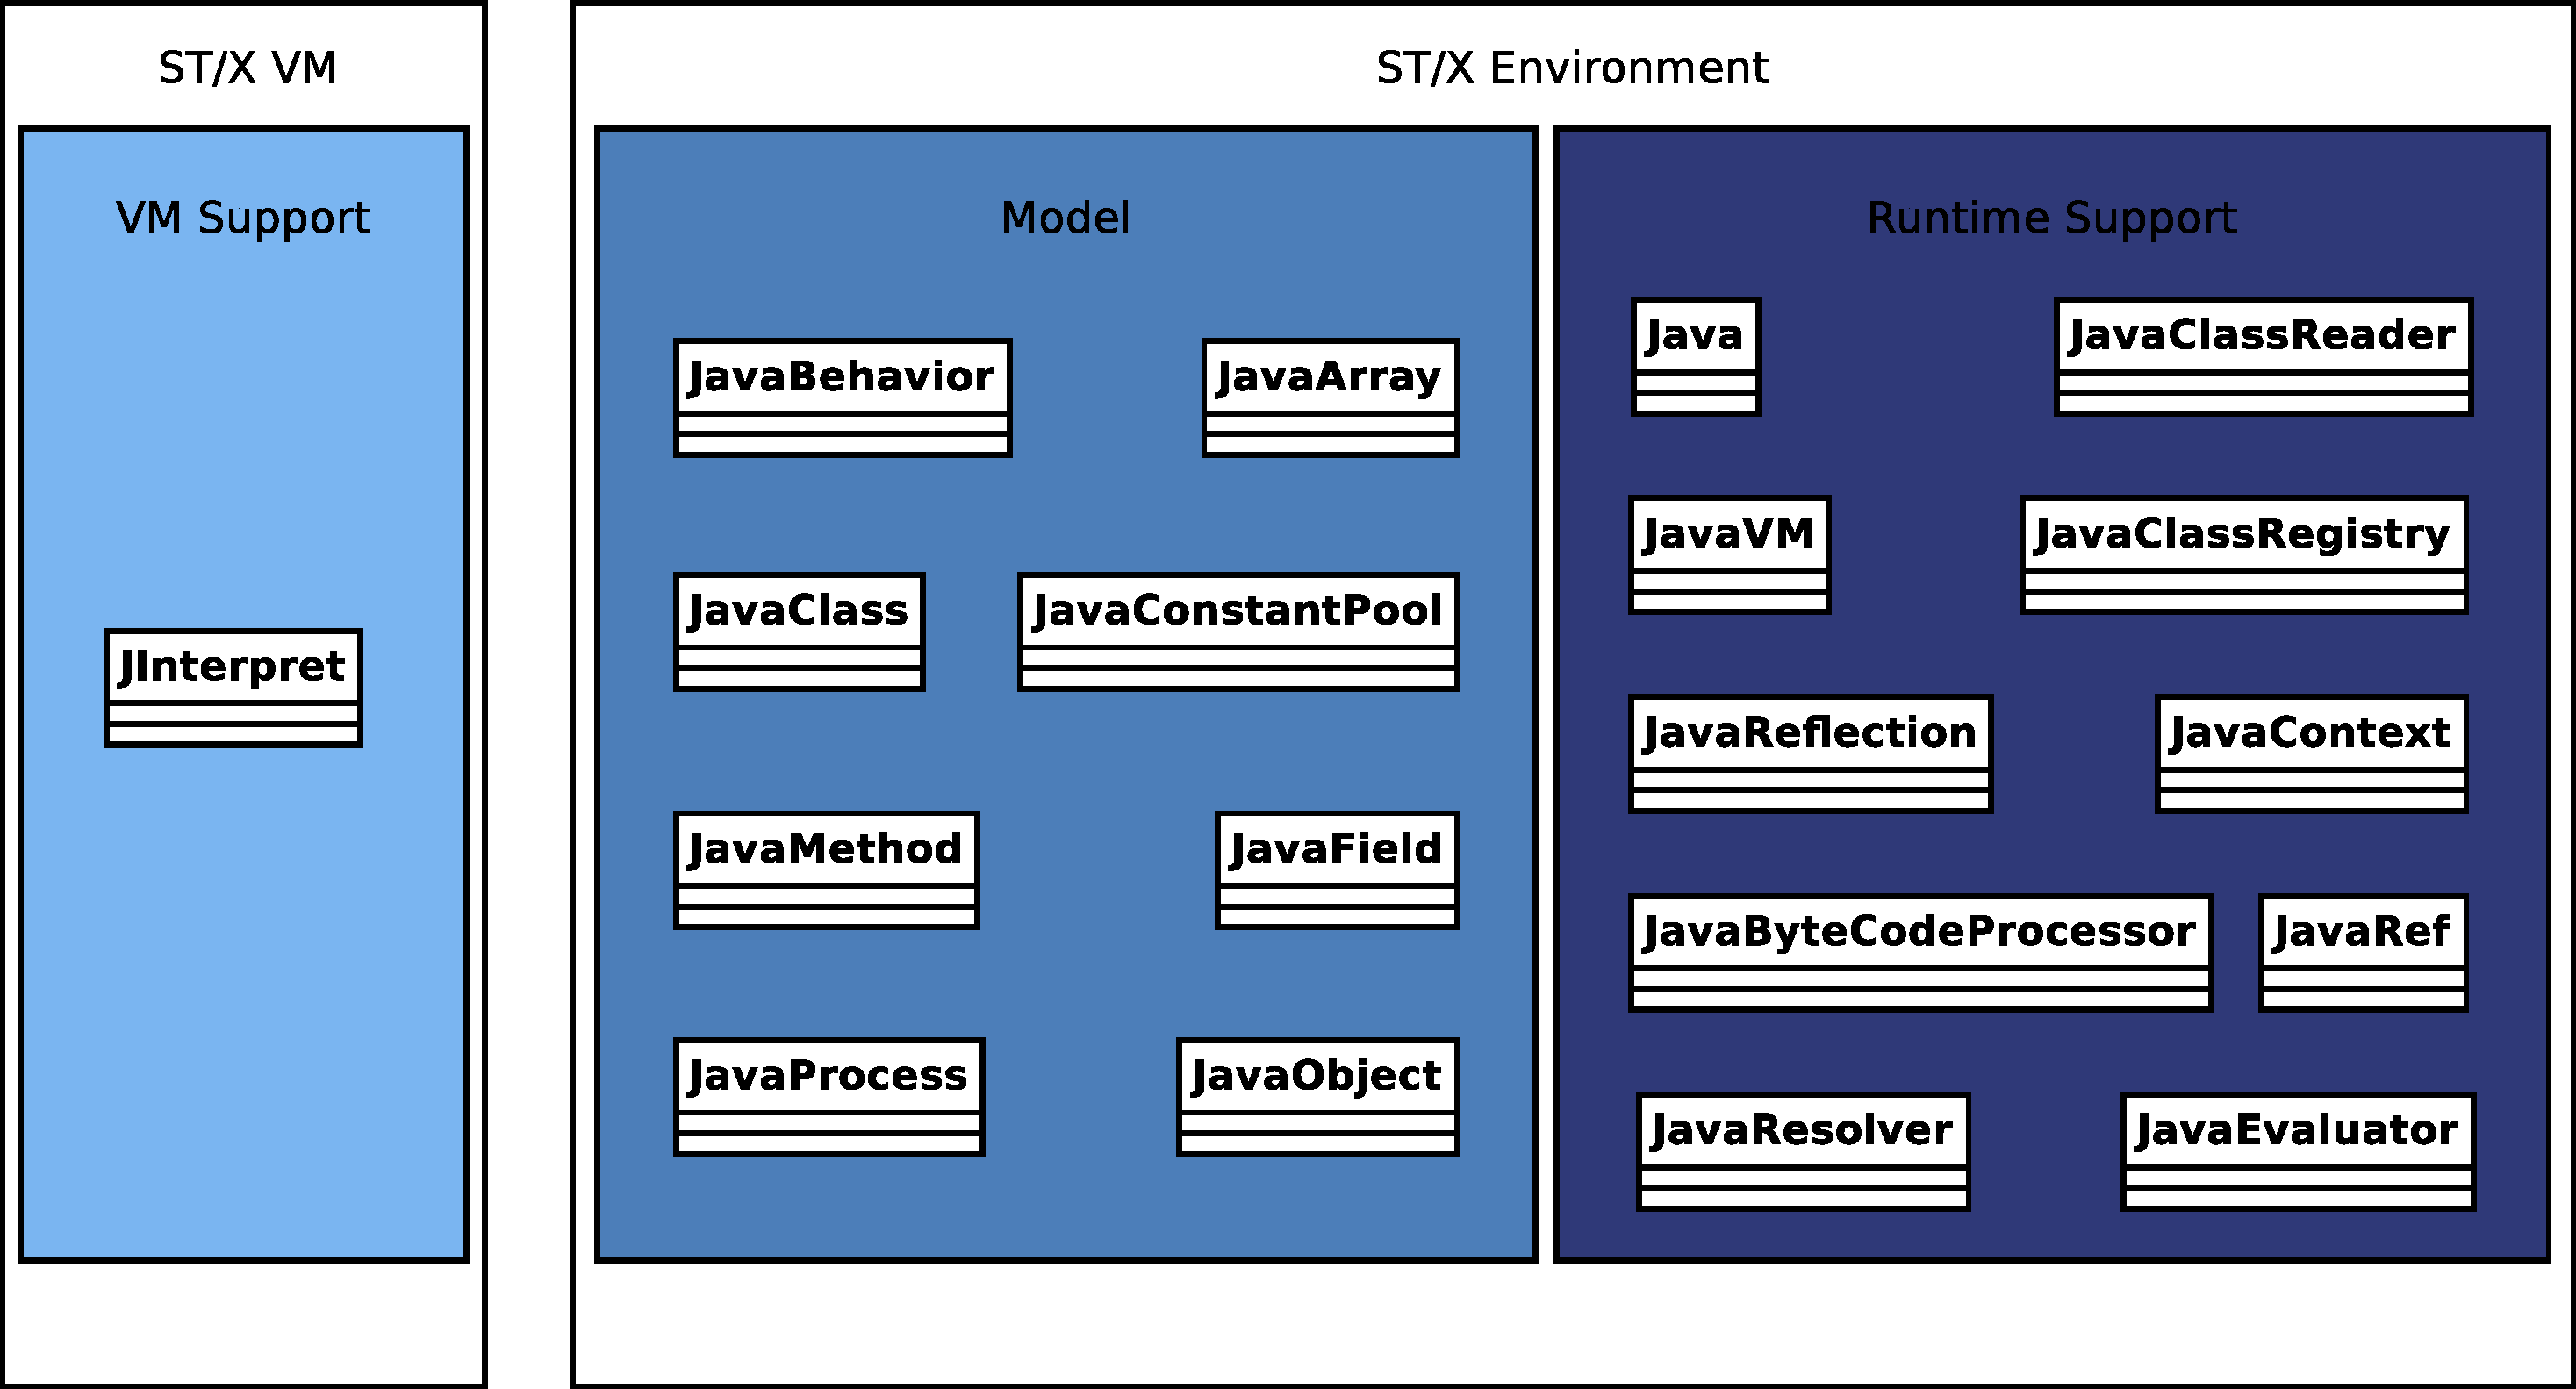
\includegraphics[width=10cm]{figures/libjava_world.pdf}
  \end{figure}
\end{frame}

\begin{frame}
	\frametitle{Hands on - Groovy}
	\putat{180}{-0}{
\includegraphics[width=5cm]{figures/groovy.png}}
    \pause
	\putat{-30}{-80}{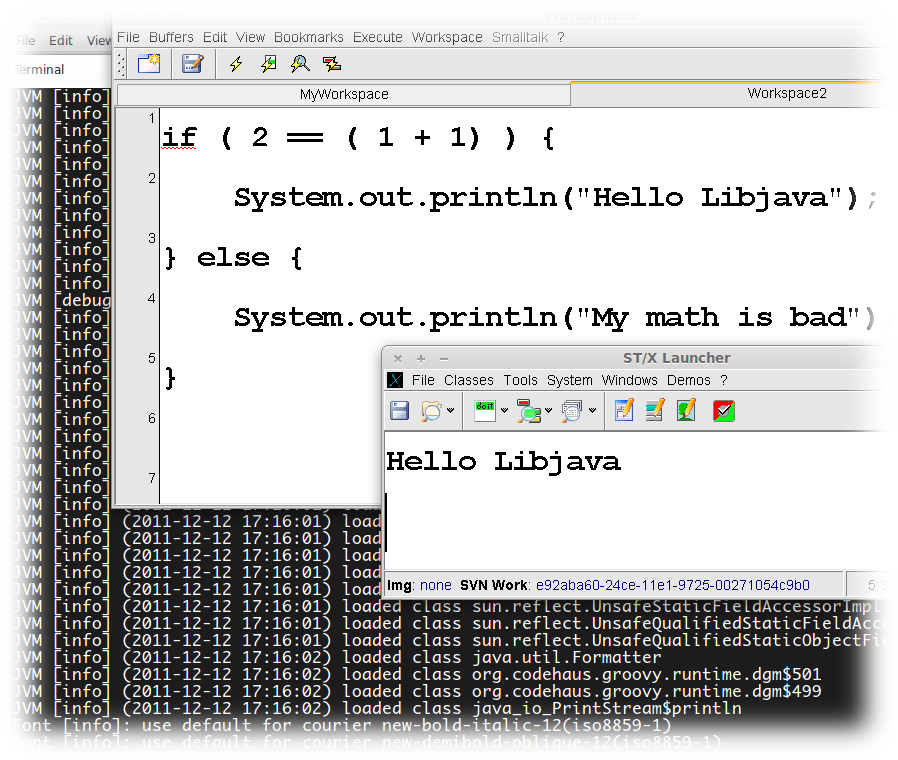
\includegraphics[width=7cm]{figures/groovy-sshot.png}}
	\pause

	\putat{0}{-89}{{\wtftext{Ok, better, but still..}}}
\end{frame}

\begin{frame}
	\fullsizegraphic{-1cm}{-2,5cm}{figures/obstaclesb.png}
	\frametitle{Obstacles on the way}
	\begin{itemize}
		\item Class Loaders \pause
		\item Synchronization \pause
		\item Exceptions \pause
		\item finally
	\end{itemize}
\end{frame}

\begin{frame}
	\putat{220}{-100}{
\includegraphics[width=4cm]{figures/tomcat.png}}
	\frametitle{Hands on - Tomcat}
    \pause
	\putat{-30}{-100}{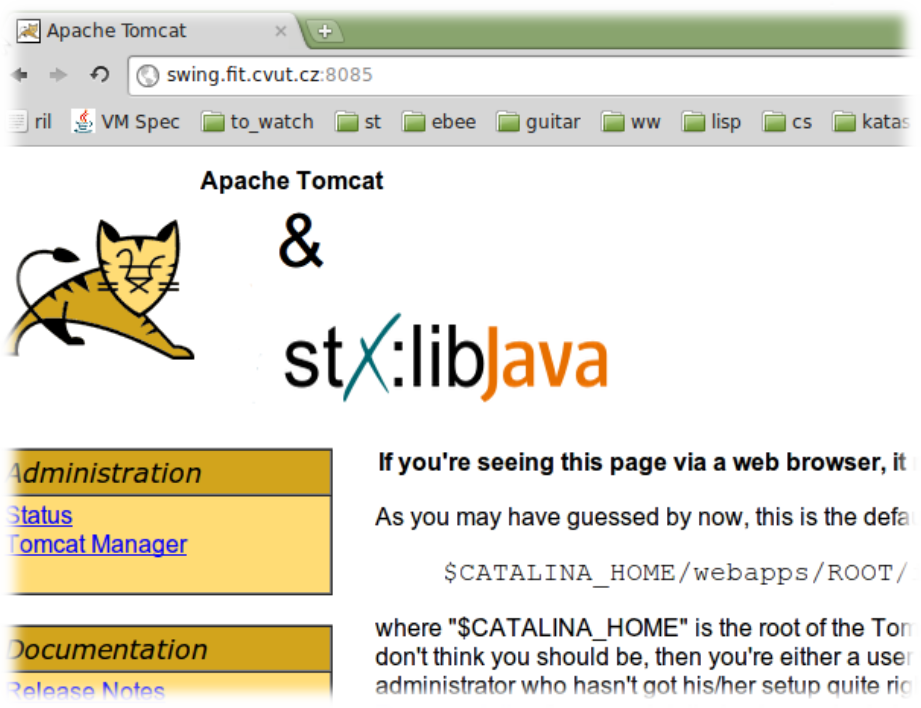
\includegraphics[width=9cm]{figures/tomcat-sshot.png}}
\end{frame}

\begin{frame}
	\fullsizegraphic{-1cm}{-25pt}{figures/cogsb.png}
	\frametitle{Bits missing -- future work}
	\begin{itemize}
		\item JIT \pause
		\item Integration \pause 
		\item Incremental compiler \pause
	\end{itemize}
	 but mostly
	 {\yeahtext{interoperability}}
\end{frame}

\begin{frame}
	\frametitle{Questions}
	\putat{210}{-100}{
\includegraphics[width=4cm]{figures/tomcat-on-smalltalk.png}}
	\begin{center}
		{\yeahtext{Q \& A}}
	\end{center}
\end{frame}

% \begin{frame}
% 	%\frametitle{Hope you enjoyed the talk}
% 	\begin{center}
% 	{\yeahtext{Thank you}}
% 	\end{center}
% \end{frame}

\end{document}

